\documentclass[tikz,border=4pt]{standalone}
\usepackage{amsmath,amssymb}
\usetikzlibrary{arrows.meta,calc,decorations.markings}
\begin{document}
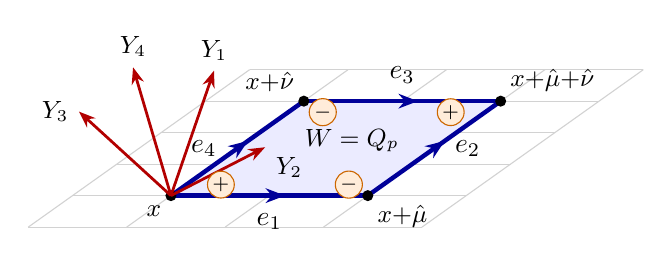
\begin{tikzpicture}[x={(1.0cm,0cm)},y={(0.45cm,0.32cm)},z={(0cm,1.0cm)},scale=1.25,
  link/.style={line width=1.6pt,draw=blue!60!black,
     postaction={decorate,decoration={markings,mark=at position 0.58 with {\arrow{Stealth[length=7pt]}}}}},
  vec/.style={-{Stealth[length=6pt]},line width=1pt,draw=red!70!black}]
% background lattice plane
\foreach \i in {-1,0,1,2,3}{\draw[gray!35] (\i,-1,0)--(\i,4,0);}
\foreach \j in {-1,0,1,2,3,4}{\draw[gray!35] (-1,\j,0)--(3,\j,0);}
\fill[blue!8] (0,0,0)--(2,0,0)--(2,3,0)--(0,3,0)--cycle;
\draw[link] (0,0,0)--(2,0,0);
\draw[link] (2,0,0)--(2,3,0);
\draw[link] (0,3,0)--(2,3,0);
\draw[link] (0,0,0)--(0,3,0);
\node[below=3pt] at (1,0,0) {$e_1$};
\node[right=4pt] at (2,1.5,0) {$e_2$};
\node[above=3pt] at (1,3,0) {$e_3$};
\node[left=4pt] at (0,1.5,0) {$e_4$};
\foreach \p/\l/\a in {(0,0,0)/x/below left,(2,0,0)/x{+}\hat\mu/below right,(2,3,0)/x{+}\hat\mu{+}\hat\nu/above right,(0,3,0)/x{+}\hat\nu/above left}
  {\fill \p circle (1.6pt); \node[\a,font=\small] at \p {$\l$};}
% tangent vectors lifted
\draw[vec] (0,0,0)--(0.55,-0.25,1.35) node[above,font=\small]{$Y_1$};
\draw[vec] (0,0,0)--(1.25,-0.65,0.7) node[below right,font=\small]{$Y_2$};
\draw[vec] (0,0,0)--(-0.8,-0.3,0.95) node[left,font=\small]{$Y_3$};
\draw[vec] (0,0,0)--(-0.25,-0.3,1.4) node[above,font=\small]{$Y_4$};
% corner markers
\foreach \p/\s in {(0.35,0.35,0)/+,(1.65,0.35,0)/-,(1.65,2.65,0)/+,(0.35,2.65,0)/-}
  {\node[circle,draw=orange!80!black,fill=orange!15,inner sep=0.6pt,font=\scriptsize] at \p {$\s$};}
\node[font=\small,align=center] at (1.05,1.75,0) {$W=Q_p$};
\end{tikzpicture}
\end{document}
